\documentclass[9pt]{beamer}
\usetheme{Boadilla}

\makeatother
\setbeamertemplate{footline}
{
	\leavevmode%
	\hbox{%
		\begin{beamercolorbox}[wd=.4\paperwidth,ht=2.25ex,dp=1ex,center]{author in head/foot}%
			\usebeamerfont{author in head/foot}\insertshortauthor
		\end{beamercolorbox}%
		\begin{beamercolorbox}[wd=.6\paperwidth,ht=2.25ex,dp=1ex,center]{title in head/foot}%
			\usebeamerfont{title in head/foot}\insertshorttitle\hspace*{3em}
			\insertframenumber{} / \inserttotalframenumber\hspace*{1ex}
	\end{beamercolorbox}}%
	\vskip0pt%
}
\makeatletter
\setbeamertemplate{navigation symbols}{}


\usepackage{lipsum}
\usepackage{appendixnumberbeamer}

\usepackage[authoryear]{natbib}
\usepackage[latin1]{inputenc}
\usepackage[T1]{fontenc}
\usepackage{caption}
\usepackage{amsmath, amssymb}
\usepackage{epstopdf}
\usepackage{graphicx}
\usepackage{lmodern}
\usepackage{xcolor}
\usepackage{xpatch}
\usepackage{multirow}
\usepackage{tikz}

\usepackage{amsmath,theorem,amssymb,graphicx, pgfplots, tabularx, placeins}
\usepackage{dsfont}
\usepackage{caption}
%\usepackage{subcaption}
%\usepackage{subcaption}
\setbeamertemplate{caption}{\raggedright\insertcaption\par}
%\setbeamertemplate{footline}[frame number]
\usepackage{csquotes}
\usepackage{bm}
\bibliographystyle{econometrica}
\usepackage[normalem]{ulem}

\usepackage{setspace}


\definecolor{gray(x11gray)}{rgb}{0.75, 0.75, 0.75}


\newcommand{\bit}{\begin{itemize}}
	\newcommand{\eit}{\end{itemize}}
\newcommand{\ben}{\begin{enumerate}}
	\newcommand{\een}{\end{enumerate}}

\newcommand{\bc}{\color{blue}}
	\newcommand{\rc}{\color{red}}


\newcommand{\lb}{\label}
\newcommand{\re}{\eqref}

\title[Frictional labor markets: basics]{Macroeconomics II, Lecture VII:\\
	 Frictional labor markets: basics}
\author{Erik {\"O}berg}
\date{}

\begin{document}

\begin{frame}
\maketitle
\end{frame}

\section{Introduction}


\begin{frame}{Introduction}

\bit
\setlength\itemsep{1.5em}

\item Lectures I-VI: frameworks for business cycle analysis

\item We learned a lot, but the models we considered had several problems, and are obviuously to stylized to understand to speak to many macroeconomic phenomena

\item In particular, two assumptions seemed very unrealistic while also important for understanding macro dynamics 
\ben
\setlength\itemsep{0.5em}
	\item Labor markets are frictionless
	
	\item Household have access to complete asset markets (and can therefore be summarized by a representative agent)
\een 

\item Remainder of the course introduces a set of models that relax these assumptions

\item Besides developing a deeper theory of business cycle dynamics, these models will allows us to explore an additional set of questions in macro research:
\bit
\item How do macroeconomic conditions affect inequality? And how does inequality affect macroeconomic conditions?
\eit 

\eit

\end{frame}


\begin{frame}{Remainder of course: outline}

\bit
\setlength\itemsep{2em}

\item Lectures VII-X: Frictional labor markets
\bit
\setlength\itemsep{0.5em}
\item 4 lectures

\item Digging deepering into the determinants of household income
\eit

\item Lectures XI-XIII: Incomplete asset markets 
\bit
\setlength\itemsep{0.5em}
\item 3 lectures

\item Digging deeper into the determinants of consumption-savings dynamics, taking the income process as given
\eit

\item To get us started with frictional labor market, we'll first look at a few key facts

\eit

\end{frame}

\begin{frame}{Today's agenda}

\ben
\setlength\itemsep{2em}

\item Labor market facts

\item Search models: overview

\item Mathematical Preliminaries

\item The McCall model

\een

\end{frame}

\begin{frame}

\begin{center}
	\huge Labor market facts \normalfont
\end{center}

\end{frame}




\begin{frame}{Introduction}

\bit
\setlength\itemsep{2em}

\item The labor market can be described in terms of
\bit
	\setlength\itemsep{0.5em}
	\item Stocks: hours worked, unemployment rate etc.
	
	\item Flows: job-finding rate, separation rate etc.
	
	\item Prices: wages
\eit

\item We will look at some basic facts relating to each of these categories

\item Main focus is US, but also quick glance at other OECD countries

\item Main data source: labor force surveys (US: CPS; Sweden: AKU)

\eit

\end{frame}

\begin{frame}{Stocks}

\bit
\setlength\itemsep{2em}

\item Main variables: Population N, Participation P, Hours worked H, Employed E, Unemployed U

\item In some time interval $\Delta t$, a person is
\bit
\setlength\itemsep{0.5em}
\item \bf employed \normalfont if hours worked > 0
\item \bf unemployed \normalfont if not working, available for work and actively looking for work
\item \bf participating \normalfont if employed or unemployed
\eit 

\item Hours worked per capita $h^c = \frac{H}{N}$

\item Question: how large are fluctuations in hours worked?

\eit

\end{frame}


\begin{frame}{SD(hours per capita) cross countries}



\begin{figure}
	\centering
	\includegraphics[scale=0.5]{figures/rs_2011_fig2.pdf}
	\caption*{\footnotesize Standard deviation of detrended log points, using data 1965-2008. From Rogerson-Shimer (Handbook LE 2011).}
\end{figure}

\bit
\item Fact 1: SD of cyclical fluctuations $\sim$ 1.5-2 percent for the US
\item Fact 2: considerable heterogeneity in fluctations across countries
\eit

\end{frame}


\begin{frame}{Decomposition}

\bit
\setlength\itemsep{1.5em}

\item More definitions
\bit
	\setlength\itemsep{0.5em}
\item Hours worked per worker $h^w = \frac{H}{E}$
%\item Participation rate $p = \frac{P}{N}$
\item Employment rate $e = \frac{E}{N}$ 
%\item Unemployment rate $u = \frac{U}{P}$
\eit

\item Decomposing hours worked
\begin{eqnarray}
h^c_t &=& \frac{H_t}{N_t} \nonumber \\
&=& \frac{H_t}{E_t} \times \frac{E_t}{N_t} \nonumber \\
&=& \underbrace{h^w_t}_{\text{int. margin}} \times \underbrace{e_t}_{\text{ext. margin}} \nonumber
\end{eqnarray}

\item Question: How much of fluctuations in hours worked per person is due to intensive vs extensive margin?

\eit

\end{frame}


\begin{frame}{SD($h^w_t$)/SD($e_t$) cross countries}



\begin{figure}
	\centering
	\includegraphics[scale=0.45]{figures/rs_2011_fig3.pdf}
	\caption*{\footnotesize Standard deviation of detrended log points, using data 1965-2008. From Rogerson-Shimer (Handbook LE 2011).}
\end{figure}

\bit
\item Fact: for most countries, extensive margin is more important (but still considerable variation due to intensive margin)
\eit

\end{frame}


\begin{frame}{Further decomposition}

\bit
\setlength\itemsep{1.5em}

\item Even more defintions
\bit
	\setlength\itemsep{0.5em}
	\item Participation rate $p = \frac{P}{N}$
	\item Unemployment rate $u = \frac{U}{P}$
\eit

\item Decomposing hours worked
\begin{eqnarray}
h^c_t &=& \frac{H_t}{E_t} \times \frac{E_t}{N_t} \nonumber \\
&=& h^w_t \times \frac{P_t-U_t}{N_t} \nonumber \\
&=& h^w_t \times \frac{P_t}{N_t} \times (1-\frac{U_t}{P_t}) \nonumber \\
&=& h^w_t \times p_t \times (1-u_t) \nonumber
\end{eqnarray}

\item Question: How much of fluctuations in hours worked is due to participation vs. unemployment?

\eit

\end{frame}


\begin{frame}{US time series}



\begin{figure}
	\centering
	\includegraphics[scale=0.5]{figures/rs_2011_fig1.pdf}
	\caption*{\footnotesize Detrended log points. Blue solid - hours worked per person; red dashed - employment rate; green dotted - participation rate. From Rogerson-Shimer (Handbook LE 2011).}
\end{figure}

\bit
\item Fact: In the US, participation accounts only marginally for cyclical variation in hours worked
\item $\Rightarrow$ most cyclical variation in hours worked is due to unemployment
\eit

\end{frame}



\begin{frame}{Flows}

\bit
\setlength\itemsep{1.5em}

\item To gain further insight about the forces behind these fluctuations, we study the underlying flows
\bit
	\item Participation fairly constant, so we restrict attention to flows in and out of unemployment
\eit

\item Denote $F_{t}(\Delta t), S_{t}(\Delta t)$ as the job-finding and job-separation probabilities in period $t \rightarrow t+\Delta t$
\bit
	\setlength\itemsep{0.5em}
	\item $F_{t}(\Delta t) = $ the fraction of unemployed flowing out of unemployment in period $t \rightarrow t+\Delta t$
	\item $S_{t}(\Delta t) = $ the fraction of employed flowing into unemployment in period $t \rightarrow t+\Delta t$
\eit

\item Graphical representation:
\begin{figure}[h]
	\begin{center}
		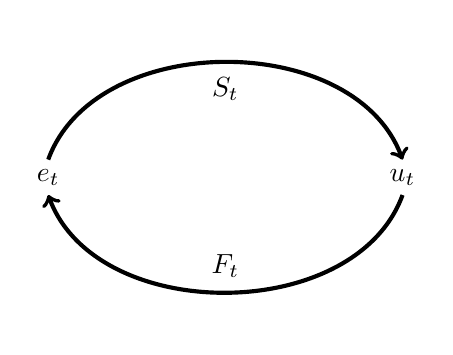
\begin{tikzpicture}[scale=0.45]		
		\draw (14,8) node{$u_t$};
		\draw (4,8) node{$e_t$};
		
		\draw (9,10.5) node{$S_t$};
		\draw (9,5.5) node{$F_t$};
		
		\draw[line width=1.5pt, ->](4,8.5) to [bend left=70] (14,8.5);
		\draw[line width=1.5pt, <-](4,7.5) to [bend right=70] (14,7.5);
		\end{tikzpicture}
	\end{center}
\end{figure}

\eit

\end{frame}

\begin{frame}{Measurement}

\bit
\setlength\itemsep{2em}

\item Assume $\Delta t = 1$ month

\item With data on unemployment levels by duration, we estimate the probability $F_t$ for an unemployed worker for finding a job within a month:
\begin{eqnarray}
1-F_t = \frac{\text{\#Unemployed with duration>1 in month t+1}}{\text{\#Unemployed in month t}} \nonumber
\end{eqnarray}

\item Similary, the monthly job-separation probability can be estimated from
\begin{eqnarray}
S_t = \frac{\text{\#Unemployed with duration<1 in month t+1}}{\text{\#Employed in month t}} \nonumber
\end{eqnarray}

\eit

\end{frame}




\begin{frame}{US job-finding probability}



\begin{figure}
	\centering
	\includegraphics[scale=0.5]{figures/rs_2011_fig6a.pdf}
	\caption*{\footnotesize Blue solid line: inference from 2-state model; Red dashed line: inference from 3-state model. Rogerson-Shimer (Handbook LE 2011).}
\end{figure}

\bit
%	\item $F_t \approx 0.45 \Rightarrow \lambda_{t} \approx 0.6$ (but lower if considering additional state)
	\item Fact: Job-finding probability decreases (somewhat gradually) during recessions
\eit

\end{frame}


\begin{frame}{US job-separation probability}



\begin{figure}
\centering
\includegraphics[scale=0.5]{figures/rs_2011_fig6b.pdf}
\caption*{\footnotesize Blue solid line: inference from 2-state model; Red dashed line: inference from 3-state model. From Rogerson-Shimer (Handbook LE 2011).}
\end{figure}

\bit
%	\item $S_t \approx 0.03 \Rightarrow \lambda_{ut} \approx 0.03$ (but lower if considering additional state)
	\item Fact: Job-separation probability spikes during recessions
\eit

\end{frame}


\begin{frame}{Flows across countries}



\begin{figure}
	\centering
	\includegraphics[scale=0.6]{figures/ehs_2013_fig1.pdf}
	\caption*{\footnotesize From Elsby-Hobjin-Sahin (ReStat 2013).}
\end{figure}

\bit
\item Fact: US labor market is an outlier

\item Fact: Strong positive association between job-separation and job-finding probability across countries
\eit

\end{frame}





\begin{frame}{Wages}

\bit
\setlength\itemsep{2em}
\item The allocation of labor is coordinated via the labor price system, that is, the wage distribution

\item How large are fluctations in wages?

\item Are different workers paid different wages? 

\item Are similar workers paid different wages?

\eit

\end{frame}

\begin{frame}{US wage fluctuations}

\begin{figure}
	\centering
	\includegraphics[scale=0.4]{figures/wages_prod.pdf}
	\caption*{\footnotesize Detrended (HP-filter) quarterly data. OECD estimate of total labor productivity. Average hourly earnings for total private sector excluding supervisory employees, deflated with PCE. Source: FRED and own calculations.}
\end{figure}

\bit
\item Fact: wage fluctuations $<<$ productivity fluctuations
\item Seemingly at odds with benchmark neoclassical model
\eit


\end{frame}



\begin{frame}{US wage dispersion}

\begin{figure}
	\centering
	\includegraphics[scale=0.5]{figures/acemoglu_2002_fig2.pdf}
	\caption*{\footnotesize From Acemoglu (JEL 2002).}
\end{figure}

\bit
\item Fact: rising wage inequality since mid-seventies
\eit


\end{frame}

\begin{frame}{Residual wage dispersion}

\bit
\setlength\itemsep{1.5em}
\item How much of the observed wage dispersion is due to the differences in observables?

\item Cross-sectional household survey data (e.g. PSID, CPS)

\item Mincer regression
\begin{eqnarray}
\log y_{it} = \mu_y + \beta \mathbf{X}_{it} + \epsilon_{it} \nonumber
\end{eqnarray}
where $y_{it}$ is earnings and $\mathbf{X}_{it}$ includes the age, occupation, industry, tenure, education etc.

\item Typically, $R^2<0.3$ (Mortensen, Book 2003)

\item How to interpret the residual $\epsilon_{it}$?
\bit
	\item Unobservable productivity differences? Luck?
\eit

\eit

\end{frame}




\begin{frame}{US residual wage dispersion}

\begin{figure}
	\centering
	\includegraphics[scale=0.45]{figures/acemoglu_2002_fig3.pdf}
	\caption*{\footnotesize Y-axis: log points. From Acemoglu (JEL 2002).}
\end{figure}

\bit
	\item In 1995, median is $\sim e^{0.6} \approx 1.8$ times 10th percentile
	\item In 1995, 90th percentile is $\sim e^{2*0.6} \approx 3.3$ times 10th percentile
	\item $\Rightarrow$ Fact: high and rising residual wage inequality
\eit


\end{frame}



\begin{frame}

\begin{center}
	\huge Search models: overview \normalfont
\end{center}

\end{frame}


\begin{frame}{Search models}

\bit
\setlength\itemsep{1.5em}

\item Search models provide a theory of the labor market that links stock, flows and the distribution of wages together

\item Search markets: markets in which buyers (employers) and sellers (workers) spend time/resources searching for each other and where there is some element of randomness in when and/or for whom a match happens 

\item Because searching takes time, some workers will experience periods without work: {\color{blue}fricitional unemployment}

\item Because matching has an element of randomness, some workers will be more lucky than others in finding good jobs: {\color{blue}fricitional wage dispersion}


\item Contrast to Walrasian markets (e.g. standard RBC and NK models)
\bit
\setlength\itemsep{0.5em}
	\item Markets clear instantaneously
	\item Unemployment can only arise if wages are not clearing the market
	\item Law of one price holds: no wage dispersion among identical workers 
\eit
 
\eit

\end{frame}


\begin{frame}{Search models}

\bit
\setlength\itemsep{1.5em}

\item The search approach to labor markets were developed in the 60's, first largely focused on partial equilibrium search behavior, later built into general equilibrium frameworks	

\item We will cover
\bit
\setlength\itemsep{0.5em}
\item Lecture VII: Partial-equilibrium search (McCall)
\item Lecture VIII: Job-ladders and wage dispersion (Burdett-Mortensen)
\item Lecture IX-X: Unemployment (Diamond-Mortensen-Pissarides)
\eit 
\eit

\end{frame}


\begin{frame}

\begin{center}
	\huge Mathematical Preliminaries \normalfont
\end{center}

\end{frame}

\begin{frame}{Math preliminaries I: Expected value}

\bit
\setlength\itemsep{1.5em}

\item For a non-negative random variable $x$ with cdf $F(x)$ on support $[x_1, x_2]$, we can define expected value as 
\begin{eqnarray}
Ex = \int_{x_1}^{x_2} x d F(x) \nonumber
\end{eqnarray}

\item Contrast with ``standard'' defintion
\begin{eqnarray}
Ex = \int_{x_1}^{x_2} x f(x)dx \nonumber
\end{eqnarray}

\item For distributions where $F$ is differentiable, these definitions coincide.  
\bit
\setlength\itemsep{0.5em}
\item $\frac{d F(x)}{d x} = f(x) \Leftrightarrow dF(x) = f(x)dx$

\item This includes the usual suspects: Uniform, Normal, Frechet, Pareto, etc... 
\eit

\item However, when $F$ has mass points, the expected value does not exist according to latter definition {\rc (Draw example on whiteboard)}

\item Hence, we will employ the former definition

\eit
\end{frame}


\begin{frame}{Math preliminaries II: Riemann-Stieltjes integrals}

\bit
\setlength\itemsep{2em}

\item Consider our definition or expected value
\begin{eqnarray}
Ex = \int_{x_1}^{x_2} x d F(x) \nonumber
\end{eqnarray}

\item When the integrator is a function rather than a variable, we call it a {\bc Riemann-Stieltjes integral}

\item Properties or RS integrals:
\ben
\setlength\itemsep{1em}
\item If $F$ is differentiable: $\int G(x) dF(x) = \int G(x) f(x) dx$

\item Integration by parts: $\int_{a}^{b} G(x) dF(x) = G(x)F(x)|_{a}^{b} - \int_{a}^{b} F(x) dG(x)$

\item In particular: $\int_{a}^{b} dF(x) = F(x)|_{a}^{b}$ 
\een

\item {\rc (Compute $Ex$ of example distribution on whiteboard)} 

\eit
\end{frame}

\begin{frame}{Math preliminaries III: Two useful formulas for real analysis}

\bit
\setlength\itemsep{2em}

\item {\bc l'H\^{o}pital's rule}: if $f(x)$ and $g(x)$ are two differentiable functions (in an open interval around $c$) and
\begin{eqnarray}
\lim\limits_{x \rightarrow c} f(x) = \lim\limits_{x \rightarrow c} g(x) = 0 \text{ or } \pm \infty \nonumber
\end{eqnarray}
then
\begin{eqnarray}
\lim\limits_{x \rightarrow c} \frac{f(x)}{g(x)}= \lim\limits_{x \rightarrow c} \frac{f'(x)}{g'(x)} \nonumber
\end{eqnarray}

\item {\bc Leibniz' rule}: If the functions $f(x,t), \alpha(t), \beta(t)$ are differentiable in $t$, the function
\begin{eqnarray}
\phi(t) = \int_{\alpha(t)}^{\beta(t)} f(x,t) dg(x) \nonumber
\end{eqnarray}
is differentiable and
\begin{eqnarray}
\phi'(t) = f(\beta(t),t) \frac{dg(\beta(t))}{dt} - f(\alpha(t),t)\frac{dg(\alpha(t))}{dt} + \int_{\alpha(t)}^{\beta(t)} f_t(x,t) dg(x) \nonumber
\end{eqnarray}

\eit
\end{frame}



\begin{frame}

\begin{center}
	\huge The McCall model \normalfont
\end{center}

\end{frame}


\begin{frame}{The McCall (QJE 1970) model}

\bit
	\setlength\itemsep{2em}
	
	\item Framework for thinking about optimal search behavior
	
	\item Identical households, who search for employment opportunities
	
	\item Partial equilibrium: we take prices (and firm behavior) as given
\eit

\end{frame}


\begin{frame}{McCall agenda}

\ben
\setlength\itemsep{1.5em}
\item Model setup

\item Reformulation of model in continuous time

\item Solution: reservation wage strategy

\item Implications:
\bit
\item Match quality
\item Unemployment duration
\item Unemployment dynamics
\item Wage dispersion
\eit

\item The Rothschild critique and the Diamond paradox
\een

\end{frame}





\begin{frame}{McCall assumptions}

\bit
\setlength\itemsep{1.5em}

\item An economy populated by a measure $P$ of ex ante identical, infinitely lived agents with linear utility function and discount factor $\beta$

\item Households can either be {\bc employed} or {\rc unemployed}

\item An {\rc unemployed} household recieves benefits {\rc $b$}, an {\bc employed}  household recieves wage {\bc$w$}

\item No savings technology, agents consume hand-to-mouth

\item Unemployed household recieve job offer with probability $\Lambda_{u}$ in each period, with wages $w$ drawn from i.i.d. $F(w)$ with finite support $\mathds{W}=[ w_{min}, w_{max}]$   

\item Employed households separate from jobs at exogenous probability $S$

\item Household problem: if unemployed and recieve job offer, accept or wait 
\eit

\end{frame}


\begin{frame}{Value functions}

\bit
\setlength\itemsep{2em}

\item Search models: generally easier to work with {\bc recursive formulation}

\item Value (i.e. Present-Discounted Value) of employed agent:
\begin{eqnarray}
W(w) =  w + \beta \left[(1-S)W(w) + S U \right] \nonumber
\end{eqnarray}

\item Value of unemployed agent:
\begin{eqnarray}
U = b + \beta \left[(1-\Lambda_{u}) U + \Lambda_{u} \int_{\mathds{W}} \max\{W(w), U\} dF(w) \right] \nonumber
\end{eqnarray}

\eit
\end{frame}





\begin{frame}{Value functions in continuous time}

\bit
\setlength\itemsep{1.5em}

\item Given these Bellman equations, we could proceed to solve for the worker decision and derive all results

\item However, many macro-search models are formulated in continuous time

\item We will therefore restate the previous problems in continuous time and work with this formulation from now on

\item Same setup, but we denote the time period by $\Delta t$ (and do not normalize it to $1$)

\item For given $\Delta t$, we distinguish between {\bc rates} and {\rc levels}
\bit
\setlength\itemsep{0.5em}
\item Job-finding rate $\lambda_u$; Job-finding probability ${\rc\Lambda_{u}(\Delta t)} = {\bc\lambda_u} \Delta t$

\item Job-separation rate $\sigma$; Job-separation probability ${\rc S(\Delta t)} = {\bc\sigma}  \Delta t$

\item Discount rate $r$; Discount factor ${\rc \beta (\Delta t)} = e^{-{\bc r} \Delta t} \approx \frac{1}{1+ {\bc r}\Delta t}$
\eit

%\item $b, w$ are instantaneous benefit and wage levels. In time period $\Delta t$, you get wage payments $w \Delta t$
%
%\item $\lambda_u, \sigma$ are instantaneous job-finding and separation probabilities 

\eit


\end{frame}

\begin{frame}{Employed value function in continuous time}

\bit
\setlength\itemsep{1.5em}

\item PDV of employed agent
\begin{eqnarray}
W(w) = w \Delta t + e^{-r \Delta t} \left[(1-\sigma  \Delta t )W(w) + \sigma  \Delta t  U \right]\nonumber
\end{eqnarray}
\item Rearrange
\begin{eqnarray}
\frac{1-e^{-r \Delta t}}{\Delta t}W(w) = w + \sigma e^{-r \Delta t}(U-W(w))\nonumber
\end{eqnarray}
\item l'H\^{o}pital's rule says
\begin{eqnarray}
\lim\limits_{\Delta t \rightarrow 0}\frac{1-e^{-r \Delta t}}{\Delta t} = \lim\limits_{\Delta t \rightarrow 0}\frac{re^{-r \Delta t}}{1} = r \nonumber
\end{eqnarray}
\item so in the limit $\Delta t \rightarrow 0$:
\begin{eqnarray}
r W(w) = w + \sigma (U-W(w)) \nonumber
\end{eqnarray}

\item flow value $rW$ $=$ flow benefit $+$ flow probability of shock $\times$ change in value

\eit


\end{frame}

\begin{frame}{Unemployed value function in continuous time}

\bit
\setlength\itemsep{1.5em}
\item PDV of unemployed agent:
\begin{eqnarray}
U &=& b \Delta t + e^{-r \Delta t} \left[(1-\lambda_u \Delta t ) U + \lambda_u \Delta t \int_{\mathds{W}} \max\{W(w), U\} dF(w)\right] \nonumber \\
&=& b \Delta t + e^{-r \Delta t} \left[U + \lambda_u \Delta t \int_{\mathds{W}} \max\{W(w)-U, 0\} dF(w)\right] \nonumber
\end{eqnarray}

\item Rearrange
\begin{eqnarray}
\frac{1-e^{-r \Delta t}}{\Delta t}U = b  + e^{-r \Delta t} \lambda_u  \int_{\mathds{W}} \max\{W(w)-U, 0\} dF(w) \nonumber
\end{eqnarray}
\item Take the limit and use l'H\^{o}pital's rule to find 
\begin{eqnarray}
rU  = b + \lambda_u  \int_{\mathds{W}} \max\{W(w)-U, 0\} dF(w) \nonumber
\end{eqnarray}

\eit
\end{frame}

\begin{frame}{Model summary}

\bit
\setlength\itemsep{2em}

\item Our problem is to find $U,W$ and a wage acceptance rule $a: \mathds{W} \rightarrow \{0,1\}$ that solves our system of two equations
\begin{eqnarray}
r W(w) &=& w + \sigma (U-W(w)) \nonumber \\ 
rU  &=&  b + \lambda_u  \int_{\mathds{W}} \max\{W(w)-U, 0\} dF(w) \nonumber
\end{eqnarray}
\item That's it

\item Now we 1) solve this problem and 2) study the implications of the solutions

\eit
\end{frame}

\begin{frame}{Solution I: the reservation wage strategy}

\bit
\setlength\itemsep{1em}

\item We solve for $W$ in terms of $U$:
\begin{eqnarray}
r W(w) = w + \sigma (U-W(w))  \Rightarrow W(w) = \frac{w+\sigma U}{r+\sigma} \nonumber 
\end{eqnarray}
\item Interpretation?

\item Using this, we rewrite unemployed value
\begin{eqnarray}
rU  &=& b + \lambda_u  \int_{\mathds{W}} \max\{\frac{w+\sigma U}{r+\sigma}-U, 0\} dF(w) \nonumber \\
&=& b + \lambda_u  \int_{\mathds{W}} \max\{\frac{w-r U}{r+\sigma}, 0\} dF(w)  \nonumber
\end{eqnarray}

\item $\frac{w-r U}{r+\sigma}$ increasing, $0$ is a constant {\bc(Draw graph on whiteboard)}

\item Ergo, the wage acceptance rule is a reservation wage strategy: accept all wages $w \geq w_R$

\item First testable hypothesis: households use {\bc reservation wage strategies}

\eit


\end{frame}

\begin{frame}{Solution II: characterizing the reservation wage strategy}

\bit
\setlength\itemsep{1.5em}

\item Because of reservation strategy, unemployed value can be rewritten
\begin{eqnarray}
rU  &=& b + \lambda_u  \int_{w< w_R} 0 dF(w) + \lambda_u  \int_{w\geq w_R} \left(\frac{w-r U}{r+\sigma} \right) dF(w) \nonumber\\
&=& b + \frac{\lambda_u}{r+\sigma}  \int_{w\geq w_R} (w-r U) dF(w) \nonumber 
\end{eqnarray}

\item The reservation wage satisfies $w_R=rU$: 
\begin{eqnarray}
w_R  -b = \frac{\lambda_u }{r+\sigma} \int_{w\geq w_R} (w-w_R) dF(w) \nonumber
\end{eqnarray}
\item We name this the {\bc reservation wage equation }
\bit
\setlength\itemsep{0.5em}
	\item LHS $=$ marginal cost of waiting

	\item RHS $=$ marginal gain of waiting 
	
	\item The equation solves for $w_R$
\eit

\item Why is $w_R>b$?

\eit
\end{frame}


%\begin{frame}{Solution III: uniqueness}
%
%\bit
%\setlength\itemsep{2em}
%
%\item LHS increasing in $w_R$, let's check if RHS is decreasing in $w_R$
%
%\item Define 
%\begin{eqnarray}
%T(w_R) = RHS = \frac{\lambda_u }{r+\sigma} \int_{w \geq w_R} (w-w_R) dF(w) \nonumber
%\end{eqnarray}
%\item Apply Leibniz's rule:
%\begin{eqnarray}
%T'(w_R) &=& \frac{\lambda_u }{r+\sigma}\left[(w_{max}-w_R)\frac{\partial F(w_{max})}{\partial w_R} - (w_{R}-w_R)\frac{\partial F(w_{R})}{\partial w_R} + \int_{w \geq w_R} -1 dF(w)        \right] \nonumber \\
%&=& -\frac{\lambda_u }{r+\sigma}\int_{w \geq w_R} dF(w) \nonumber
%\end{eqnarray}
%
%\item Ergo, $T'(w_R)<0$ and we have a unique solution
%
%\eit
%
%
%\end{frame}

\begin{frame}{Solution retrieved, what now?}

\bit
\setlength\itemsep{1.5em}

\item Reminder: The problem was to find the acceptance rule, which we have shown to be cutoff strategy with reservation wage $w_R$

\item This is all there is to it

\item Solving explicitly for $w_R$ requires knowledge about $F$

%\item Even though $F$ might be a complicated distribution, one can show that $T(w_R)$ is a contraction mapping 
%
%\item The reservation wage equation is $w_R -b= T(w_R)$ $\Rightarrow$ simple procedure to solve for $w_R$ given $F$ is to start with $w_1$, solve for $w_2 -b = T(w_1)$, $w_3 -b= T(w_2)$ and so on.

\item We will remain agnostic about $F$ here, but we can still derive a lot of properties and implications of the solution

\eit


\end{frame}




\begin{frame}{Comparative statics I}

\bit
\setlength\itemsep{1em}

\item How does $w_R$ vary with $b$? Our solution satisfies
\begin{eqnarray}
w_R  -b = T(w_R) \equiv \frac{\lambda_u }{r+\sigma} \int_{w\geq w_R} (w-w_R) dF(w) \nonumber
\end{eqnarray}
\item Differentiate w.r.t. b:
\begin{eqnarray}
\frac{dw_R}{db}  - 1 = T'(w_R) \frac{dw_R}{db} \nonumber
\end{eqnarray}
\item Rearrange:
\begin{eqnarray}
\frac{dw_R}{db} =\frac{1}{1-T'(w_R)}  \nonumber
\end{eqnarray}
\item Apply Leibniz's rule:
\begin{eqnarray}
T'(w_R) &=& \frac{\lambda_u }{r+\sigma}\left[(w_{max}-w_R)\frac{\partial F(w_{max})}{\partial w_R} - (w_{R}-w_R)\frac{\partial F(w_{R})}{\partial w_R} + \int_{w \geq w_R} -1 dF(w)        \right] \nonumber \\
&=& -\frac{\lambda_u }{r+\sigma}\int_{w \geq w_R} dF(w) \nonumber \\
&<& 0 \nonumber
\end{eqnarray}

\item Ergo, {\bc reservation wages increases with unemployment benefits}
\eit


\end{frame}


\begin{frame}{Comparative statics II}

\bit
\setlength\itemsep{1em}


\item Similarly, one can show
\begin{eqnarray}
\frac{dw_R}{d\lambda_u} > 0, \hspace{5 mm } \frac{dw_R}{d r} < 0 \nonumber, \hspace{5 mm }  \frac{dw_R}{d\sigma} < 0
\end{eqnarray}

\item Intuition?
\eit


\end{frame}


\begin{frame}{Comparative statics III}

\bit
\setlength\itemsep{2em}

\item What about changes in $F$?

\item A uniform increase in $F(w)$ increases the reservation wage

\item How does $w_R$ respond to an increase in dispersion? 
\bit
	\item see your problem set
\eit


\eit


\end{frame}

%\begin{frame}{Unemployment duration}
%
%\bit
%\setlength\itemsep{2em}
%
%\item What is expected unemployment duration in our model?
%
%\item Given an instantaneous job-finding rate $\lambda = \lambda_u (1-F(w_R))$, one can proove that $H(t) = P(\text{not found a job at time t})$ is given by
%\begin{eqnarray}
%	H(t) = e^{-\lambda t} \nonumber
%\end{eqnarray}
%
%\item The expected duration of an unemployment spell is
%\begin{eqnarray}
%D = \int_{t=0}^{\infty}H(t) dt = \int_{t}^{\infty} e^{-\lambda t} dt = \frac{1}{\lambda} \nonumber
%\end{eqnarray}
%
%\item \bf Hypothesis 3: Everything that increases $w_R$ (e.g. benefits $b$) will also increase unemployment duration \normalfont
%
%\eit
%
%
%\end{frame}


\begin{frame}{Match quality}

\bit
\setlength\itemsep{2em}

\item The observed wage distribution is $G(w; w_R) = F(w | w>w_R)$

\item An increase in $w_R$ implies that observed wages are higher

\item More precisely: if $w^1_R>w^2_R$, then $G_1(w; w^1_R)$ first order stochastically dominates $G_2(w; w^2_R)$
\bit
	\item The only difference between $G_1(w; w^1_R)$ and $G_1(w; w^2_R)$ is that lower wage offers are discarded in $G_1(w; w^1_R)$
\eit

\item {\bc Hypothesis: Everything that increases $w_R$ (e.g. benefits $b$) will also increase observed wages}

\item Reformulated: higher unemployment benefits should increase observed {\bc match quality}

\eit


\end{frame}



\begin{frame}{Unemployment dynamics}

\bit
\setlength\itemsep{1em}

\item The economy is populated with $P$ workers 

\item In a time period $\Delta t$, a fraction $\sigma \Delta t$ of employed workers $E_t = P-U_t$ separate and a fraction $\lambda\Delta t$ of unemployed workers  $U_t$ find a job
\bit
	\item $\lambda = \lambda_u (1-F(w_R))$
\eit

\item Law of motion for unemployment
\begin{eqnarray}
U_{t+\Delta t} = U_t + \sigma \Delta t (P-U_t) - \lambda \Delta t U_t \nonumber
\end{eqnarray}

\item Divide by $P$:
\begin{eqnarray}
u_{t+\Delta t} = u_t + \sigma \Delta t (1-u_t) - \lambda \Delta t u_t \nonumber
\end{eqnarray}

\item Rearrange:
\begin{eqnarray}
\frac{u_{t+\Delta t}-u_t}{\Delta t} = \sigma (1-u_t) - \lambda u_t \nonumber
\end{eqnarray}

\item Take the limit $\Delta t \rightarrow 0$:
\begin{eqnarray}
\dot u_t = \sigma (1-u_t) -\lambda u_t \nonumber
\end{eqnarray}
%
%\item This \emph{Ordinary Differential Equation of Order 1} connects the evolution unemployment to the underlying job-finding and job-separation rate

\eit


\end{frame}


\begin{frame}{Unemployment dynamics II}

\bit
\setlength\itemsep{2em}

\item {\bc Law of motion for unemployment}:
\begin{eqnarray}
\dot u_t = \sigma (1-u_t) -\lambda u_t \nonumber
\end{eqnarray}

\item Given $\sigma, \lambda$, this {\bc ordinary differential equation} has a unqiue solution converging to steady state value $u$.

\item Steady state $u$ defined by $\dot{u}_t = 0$:
\begin{eqnarray}
u = \frac{\sigma}{\sigma + \lambda} \nonumber
\end{eqnarray}

\item {\bc Hypothesis: Everything that increases $w_R$ (e.g. benefits $b$) will also increase the unemployment rate}

\item How does the unemployment rate relate to unemployment duration here?


\eit


\end{frame}


\begin{frame}{Digression: micro-level evidence of model predictions I}

\bit
\setlength\itemsep{1.5em}

\item Following these insights, large empirical literature have used micro data to investigate the effect of unemployment benefits on unemployment incidence, unemployment duration and match quality

\item Reservation wages and job-search behavior
\bit
	\setlength\itemsep{0.5em}
	\item A Krueger-Mueller (AEJep 2016) use interview data to document self-percieved reservation wages
	\item Marinescu-Skandalis (QJE 2020) use online application data to document how job-search behavior change with benefit duration
\eit

\item Unemployment duration and benefit generosity:
\bit
	\setlength\itemsep{0.5em}
	\item Older literature summarized in A Kreuger and Meyer (Handbook PE 2002)
	
	\item Card-Lee-Pei-Weber (Ecmtra, 2015) exploit kinks in Austrian UI
	
	\item Kolsrud-Landais-Nilsson-Spinnewijn (AER 2017) exploit kinks in Swedish UI
	
	\item Many more papers...
	
	\item Raj Chetty's summary: 10 weeks of extra UI $\Rightarrow$ 1 week of extra unemployment (of course, the effect depends on all kinds of things)
	
	\item Key input for evaluating optimal benefit provision: see, e.g., Chetty (JPubE, 2006), Chetty (JPE, 2008)
\eit

\eit


\end{frame}


\begin{frame}{Digression: micro-level evidence of model predictions II}

\bit
\setlength\itemsep{1.5em}


\item Match quality and benefit generosity:
\bit
	\setlength\itemsep{0.5em}
	\item van Ours-Vodopivec (JLE 2006); Lalive (AER 2007); Card-Chetty-Weber (QJE 2007); Schmieder-von Wachter-Bender (AER 2016): zero effect

	\item Nekoei-Weber (AER 2017) uses austrian micro data and RD design: positive effect
\eit

\item Lesson that appears in many of these papers: duration dependence matter
\bit
\setlength\itemsep{0.5em}
\item Reservation wage falls as unemployment benefit period is ending; human capital depreciates while unemployed
\eit

\item Ljungqvist-Sargent (JPE 1998) argue that duration dependence is key for understanding difference in unemployment dynamics in Europe vs. US
%\bit
%\setlength\itemsep{0.5em}
%\item EU labor markets characterized by more generous replacement rates than US
%
%\item Human capital depreciates over unemployment spell and replacement rate is tied to previously earned wage
%
%\item Therefore, unemployment workers can get stuck in situation where $w_R>w_{offered}$ $\Rightarrow$ long-term unemployment
%
%\item Potentially explains why Europe got stuck with persistently high level of long-term unemployment after oil-price shocks in the 70's, while US was not
%\eit

\eit


\end{frame}



\begin{frame}{Digression: Ljungqvist-Sargent (JPE 1998)}

\begin{figure}
	\centering
	\includegraphics[scale=0.6]{figures/ljungqvist_fig1.pdf}
	\caption*{\footnotesize Solid line: OECD Europe. Dashed line: OECD average.}
\end{figure}


\end{frame}


\begin{frame}{Digression: Ljungqvist-Sargent (JPE 1998)}

\bit
\setlength\itemsep{1.5em}
\item Hypothesis: human capital depreciates over unemployment spell
\bit
\setlength\itemsep{0.5em}
	\item Consistent with studies on mass layoffs: earnings losses after unemployment are very persistent (Lalonde-Jacobsen-Sullivan, AER 1993; Davis-von Wachter BPEA 2012)

	\item Evidence based on mass layoffs might confound partial and general equilibrium effects (Cederl�f 2019) - see lecture 3 on DMP model
\eit

\item In 70-80's: European countries had generous replacement rates tied to previous wage with close-to unlimited duration

\item Human capital depreciation + unlimited duration may result in $w_R>w_{offered}$ $\Rightarrow$ long-term unemployment

\item Makes little difference when macroeconomic volatility is low

\item In late 70's/80's: macroeconomic volatility increased (oil price shocks) $\Rightarrow$ difference in UI institutions can explain why Europe but not US got stuck in high (long-term) unemployment equilibrium 
\eit

\end{frame}


\begin{frame}{Frictional wage dispersion}

\bit
\setlength\itemsep{2em}

\item Because of the randomness of wage offers, models of this sort generate {\bc frictional wage dispersion}

\item Hypothesis: some of the empirical wage dispersion that cannot be accounted for by observed hetereogeneity is due to this kind of randomness

\item Remember: Mincer regression typically produce $R^2 < 0.3$ (Mortensen, Book 2003) and substantial residual dispersion: Acemoglu (JLE 2002) reports 90/10-ratio $\approx 3.3$ and 50/10-ratio $\approx 1.8$

\item Can our model account for these numbers?

\eit


\end{frame}

\begin{frame}{Frictional wage dispersion: how to the test the model?}

\bit
\setlength\itemsep{2em}

\item To answer this question, the obviuous approach seems to be
\ben
\setlength\itemsep{0.5em}
	\item match the model parameters $\{r, \lambda_u, F(w), b\}$ to the data

	\item solve for the reservation wage
	
	\item compute the wage distribution implied by the model $G(w) = F(w | w>w_R)$
	
	\item compare to the data
\een

\item Are there any problems with this approach?

\eit


\end{frame}

\begin{frame}{Frictional wage dispersion: an alternative approach}

\bit
\setlength\itemsep{1.5em}

\item Hornstein-Krusell-Violante (AER 2011): use the information implicitly contained in households' search behavior

\item Again, the reservation wage equation is:
\begin{eqnarray}
w_R  -b = \frac{\lambda_u }{r+\sigma} \int_{w\geq w_R} (w-w_R) dF(w) \nonumber
\end{eqnarray}

\item The observed mean wage is $\bar w = E [w | w > w_R]$

\item Rearrange
\begin{eqnarray}
w_R  - b = \frac{\lambda}{r+\sigma} \frac{\int_{w\geq w_R} (w-w_R) dF(w)}{1-F(w_R)} \nonumber
\end{eqnarray}
where $\lambda = \lambda_u (1-F(w_R))$ is the observed job-finding rate

\item What is the last ratio?
\eit
\end{frame}

\begin{frame}{Frictional wage dispersion: a useful formula}

\bit
\setlength\itemsep{1em}
\item Step-by-step:
\begin{eqnarray}
\frac{\int_{w\geq w_R} (w-w_R) dF(w)}{1-F(w_R)} &=& \frac{\int_{w\geq w_R} w dF(w)}{1-F(w_R)} - w_R \frac{\int_{w\geq w_R} dF(w)}{1-F(w_R)} \nonumber \\
&=& E [w | w > w_R] - w_R \frac{1-F(w_R)}{1-F(w_R)}\nonumber \\
&=& \bar w -w_R \nonumber
\end{eqnarray}
\item and so the reservation equation can be written
\begin{eqnarray}
w_R  - b = \frac{\lambda}{r+\sigma} (\bar w - w_R)\nonumber
\end{eqnarray}
\item Write $b = \rho \bar w$, divide by $w_R$ and rearrange
\begin{eqnarray}
Mm = \frac{\bar w}{w_R} = \frac{\frac{\lambda}{r+\sigma}+1}{\frac{\lambda}{r+\sigma}+\rho \nonumber}
\end{eqnarray}

\item Mm is a measure of wage dispersion and \bf the formula does not have $F$ in it! \normalfont

\item Can the model match the data?
\bit
\setlength\itemsep{0.5em}
\item All parameters in our formula are observed in the data!
\item Plug in parameter values and compare Mm ratio in model to data
\eit


\eit
\end{frame}

%\begin{frame}{Frictional wage dispersion: understanding the formula}
%
%\bit
%\setlength\itemsep{1.5em}
%
%\item What is the intuition?
%
%\item Take a step back and look at:
%\begin{eqnarray}
%w_R  - \rho \bar w = \frac{\lambda}{r+\sigma} (\bar w - w_R)\nonumber
%\end{eqnarray}
%\bit
%\setlength\itemsep{0.5em}
%	\item The job-finding rate $\lambda$ already summarizes what we need to know about the offer distribution
%	
%	\item Specifically, it tells us the probability mass above $w_R$ since $\lambda = \lambda_u (1-F(w_R))$
%	
%	\item Given $\lambda, \bar w, w_R$, we know the marginal gain of waiting $=\frac{\lambda}{r+\sigma} \times (\bar w -w_R)$
%	
%	\item Optimal behaviour tells us that this equals the marginal cost of foregoing the reservation wage $= w_r-\rho\bar w$
%\eit
%
%\item Can the model match the data?
%\bit
%\setlength\itemsep{0.5em}
%	\item All parameters in our formula are observed in the data!
%	\item Plug in parameter values and compare Mm ratio in model to data
%\eit
%
%\eit
%\end{frame}


\begin{frame}{Frictional wage dispersion: testing the model}

\bit
\setlength\itemsep{1em}

\item US monthly data: $r=0.0041$ (5\% yearly interest rate), $\sigma = 0.03$, $\lambda=0.43$, $\rho=0.41$ (average replacement rate) $\Rightarrow$

\begin{eqnarray}
Mm =  \frac{\frac{\lambda}{r+\sigma}+1}{\frac{\lambda}{r+\sigma}+\rho} =  \frac{\frac{0.43}{0.0041+0.03}+1}{\frac{0.43}{0.0041+0.03}+0.41} = 1.046 \nonumber
\end{eqnarray}

\item Reminder: 50/10-ratio in data $\approx 1.8$

\item \bf The model comes now way near the data! \normalfont

\item Intuition: high empirical $\lambda$ puts tight constraint on the value of expected wage offer
\bit
\setlength\itemsep{0.5em}
	\item High $\lambda$ $\Rightarrow$ households must think it is not worth waiting long to get a better offer
	\item $\Rightarrow$ expected wage from a new offer $\bar w$ cannot be much higher than outside option $\rho \bar w$
\eit

\item Only ingredient is optimal search behavior of households $\rightarrow$ very robust result

\item However, we shall see that one interesting avenue to think about fricitional wage dispersion is models in which households also perform on-the-job search

\eit
\end{frame}

\begin{frame}{Taking stock}

\bit
\setlength\itemsep{2em}

\item Key idea: unemployed households reject some wage offers because the option value of waiting for better offers dominates

\item Generates predictions on unemployment rate, unemployment duration, match quality, wage dispersion

\item Motivated by these predictions, large empirical literature has emerged

\item But the question that begs to be answered: where did the offer distribution $F$ and contact rate $\lambda_u$ come from?
\bit
	\item Presumably vacancy/wage posting by firms?
\eit

\item Also, we would presume that firm vacancy/wage posting behavior depends on worker search behavior, so can we really treat $F$ and $\lambda_u$ as exogenous?
\bit
	\item We need a GE model to explore this!
\eit

\eit
\end{frame}

\begin{frame}{General equilibrium? The Rothshild (JPE 1973) critique}

\bit
\setlength\itemsep{1.5em}

\item Suppose that the wage distribution $F$ is generated by wage-posting firms with different productivities $p>b$

\item Suppose that the firms know that all workers are identical and all workers follow the same reservation wage strategy (accept all $w>w_R$)

\item What is the optimal wage posting rule of the firms?

\item If posting $w>w_R$, you always get someone to work for you after a contact

\item If posting $w<w_R$, you never get someone to work for you

\item Optimal wage posting strategy is simply $w=w_R$, independent of $p$

\item $\Rightarrow F$ is degenerate with unit mass point at $w=w_R$!

\eit
\end{frame}


\begin{frame}{General equilibrium? The Diamond (JET 1971) paradox}

\bit
\setlength\itemsep{1.5em}

\item The problem goes deeper still. If there is no wage distribution, there is no point for an unemployed household to wait

\item Our reservation wage equation:
\begin{eqnarray}
w_R  -b &=& \frac{\lambda_u }{r+\sigma} \int_{w\geq w_R} (w-w_R) dF(w) \nonumber \\
&=& \frac{\lambda_u }{r+\sigma} \int_{w\geq w_R} (w_R-w_R) dF(w) \nonumber \\
&=& 0 \nonumber
\end{eqnarray}

\item Ergo, optimal search behavior implies $w_R=b$ and all firms offer the monopoly contract $w=b$

\item If workers have to pay a tiny fixed cost $\epsilon>0$ for participating in search, nobody would search for jobs and there would be no production!

\item Clearly, firm behavior and wage formation need to be addressed. Cliffhanger...
\eit
\end{frame}


\begin{frame}{Bonus material: mapping data probabilties to model flow rates}

\bit
\setlength\itemsep{1.4em}
\item How to retrieve continuous-time transition rates from discrete-time transition probabilities (which are measurable in the data)?

\item Our model says that in an interval $\delta t \rightarrow 0$
\ben
	\item you can get at most one job
	\item the probability of finding and accepting a job is $\lambda \delta t$
\een

\item Suppose we allowed workers to accept $>1$ jobs within some empirically measurable time period $\Delta t$ and that the arrival rate of job offers is independent of time
\bit
\item This does not change anything in our continuous-time model, as the probability of finding $>1$ jobs in any given instant is neglible
\eit

\item Then, the probability of finding $k$ jobs in period $\Delta t$ is $P(k | \Delta t)$, where $P$ is given by the Poisson distribution with arrival rate $\lambda$
\bit
	\item Hence, $P(k | \Delta t) = \frac{(\lambda \Delta t)^k}{k!} e^{-\lambda \Delta t}$
\eit

\item What we can measure in the data is $F_t(\Delta t)$ --- this is related to the continuous-time job-finding rate according to
\begin{eqnarray}
F_t(\Delta t) = 1- P(0 | \Delta t) = 1- e^{-\lambda \Delta t} \nonumber
\end{eqnarray}

\item \bf If $F_t$ is the monthly job-finding probability, then $\lambda = - \log(1-F_t)$ is the monthly job-finding rate \normalfont

\eit


\end{frame}

\begin{frame}{Bonus material: mapping data probabilties to model flow rates}



\begin{figure}
	\centering
	\includegraphics[scale=0.5]{figures/rs_2011_fig6a.pdf}
	\caption*{\footnotesize Blue solid line: inference from 2-state model; Red dashed line: inference from 3-state model. From Rogerson and Shimer (Handbook LE 2011).}
\end{figure}

\bit
	\item $F_t \approx 0.45 \Rightarrow \lambda_{t} \approx - \log(1-0.45) \approx 0.6$ 
\eit

\end{frame}

\end{document}





















